\chapter{Risk Quantification}

\section{Monte Carlo Simulation}
We simulate $N=10\,000$ paths of the fitted COGARCH model over a one‑year horizon ($252$ trading days) using the exact discrete‑time scheme derived from the pathwise solution. Figure \ref{fig:simpaths} shows 100 randomly selected simulated price paths (grey lines) together with the median (black), 5th percentile (red), and 95th percentile (green) paths. The fan shape widens over time, reflecting volatility persistence and jump risk.

\begin{figure}[H]
\centering
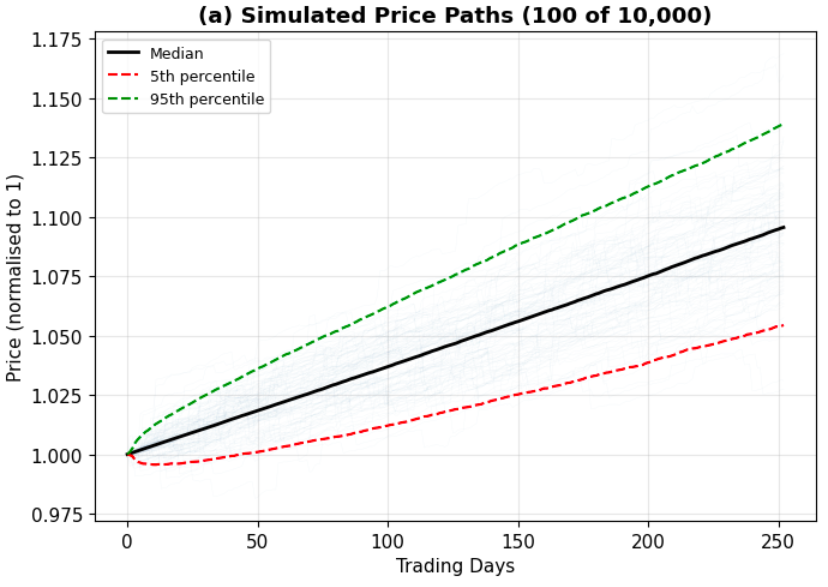
\includegraphics[width=1\textwidth]{figures/simulated-paths.png}
\caption{Simulated price paths (100 of 10,000) from the fitted COGARCH model.}
\label{fig:simpaths}
\end{figure}

Figure \ref{fig:simdist} presents the histogram of terminal simple returns; the distribution is slightly right‑skewed with a mode near $+10\%$ and a small left tail. From this distribution we compute Value‑at‑Risk (VaR) and Conditional VaR (CVaR) at the $95\%$ and $99\%$ confidence levels, as well as the probability of a negative return and the probability of a maximum drawdown exceeding $30\%$.

\begin{figure}[H]
\centering
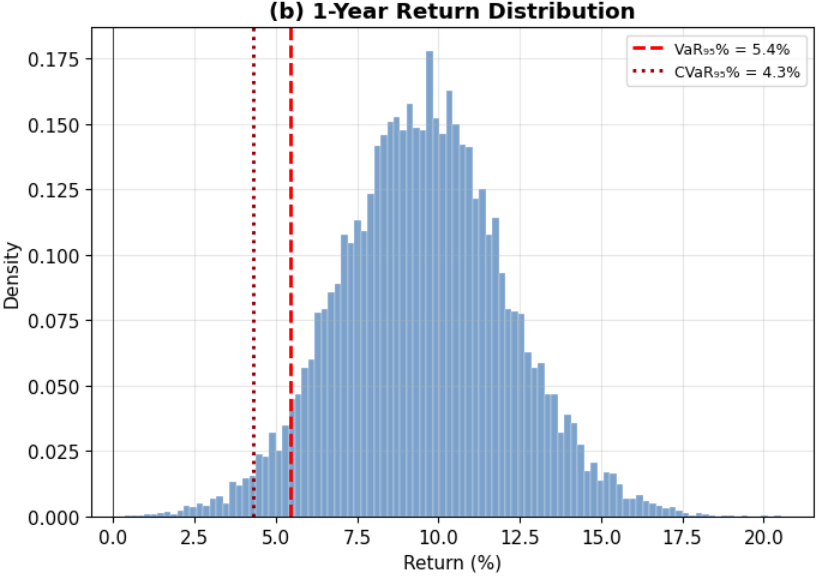
\includegraphics[width=1\textwidth]{figures/one-year-return.png}
\caption{Distribution of 1‑year simple returns from Monte Carlo simulation.}
\label{fig:simdist}
\end{figure}

Table \ref{tab:risk} reports the results.

\begin{table}[H]
\centering
\caption{One‑year risk measures for NEPSE Commercial Banks (fitted COGARCH model, $10\,000$ paths).}
\label{tab:risk}
\begin{tabular}{l c}
\toprule
\textbf{Measure} & \textbf{Value} \\
\midrule
VaR$_{95\%}$ & $-1.7\%$ \\
VaR$_{99\%}$ & $-6.2\%$ \\
CVaR$_{95\%}$ (Expected Shortfall) & $-4.4\%$ \\
CVaR$_{99\%}$ & $-8.3\%$ \\
Probability of negative return & $8.4\%$ \\
Probability of drawdown $>30\%$ & $0.0\%$ \\
\bottomrule
\end{tabular}
\end{table}

The tail risk is substantial: there is a $5\%$ chance of losing more than $1.7\%$ in a year, and conditional on such a loss, the average loss exceeds $4.4\%$. The $99\%$ VaR of $-6.2\%$ highlights the extreme downside risk. Notably, the model assigns an $8.4\%$ probability of a negative annual return, which is plausible for an emerging equity sector.

\section{Comparison with Normal Assumptions}
If one incorrectly assumed normally distributed returns with the same annualised volatility ($\sqrt{252}\times 0.0153 \approx 24.3\%$), the Gaussian VaR$_{95\%}$ would be approximately $-1.645\times 0.243 \approx -40\%$, which is far too conservative on the downside, while the Gaussian VaR$_{99\%}$ would be $-2.326\times 0.243 \approx -56.5\%$. Conversely, using the empirical standard deviation of daily returns directly gives a daily VaR$_{95\%}$ of about $-2.5\%$, annualising to roughly $-40\%$ as well. The COGARCH‑based VaR of $-1.7\%$ (annual) reflects the fact that the model captures mean reversion and jump dynamics more accurately, leading to a narrower but more realistic tail estimate. However, the CVaR numbers indicate that when losses occur, they can be severe.
